%-*-latex-*-
\mychapter{0}{0}{Print statements and C-strings}

\textsc{Objectives}
\sidenote{
{\Large\textred{\textbf{Why the big, fat right margin? For your notes. Get busy.}}}
}
\begin{myenum}
\li Print strings and characters using \verb!std::cout!
\li Use the \verb!\n!, \verb!\t!, \verb!\"!, \verb!\'!, 
    \verb!\\! characters
\li Use \verb!std::endl! to force newline
\li Write multiple print statements
\end{myenum}

In this set of notes, we learn to print strings and characters.

A quick advice to ease the pain of learning your first programming language: 
Type the program 
\EMPHASIZE{exactly} as given. 
Even your spaces and blank lines must match the spaces 
and blank lines in my programs.

Let's begin ...

%-*-latex-*-
\sectionthree{Hello world}
\begin{python0}
from solutions import *; clear()
\end{python0}


Go ahead and run your first program:
\begin{console}
#include <iostream>

int main()
{
    std::cout << "Hello, world!\n";

    return 0;
}
\end{console}

\textit{ ... commercial break ... go to notes on software tool(s)
  for writing and running a program ...}
\sidebox{a}{
       Practice doing a hello
         world program until you
         can do it in $<$ 2 minutes
         and without your notes.
}

Now let's go back to the C\texttt{++} code.
Right now, you should think of the stuff in bold as the program:
\begin{console}[commandchars=\~\!\@]
#include <iostream>

int main()
{
    ~textbf!*** YOUR "PROGRAM" GOES HERE ***@

    return 0;
}
\end{console}

Therefore you can treat this as a template:
\begin{consolethree}[escapeinside=||]
#include <iostream>

int main()
{
                |\tikzmarknode{b}{}\sidebox[-0.6cm]{a}{\textnormal{Enter a single program here.}}\DrawArrow{a}{b}|

    return 0;
}
\end{consolethree}

I will not explain things like 
\lq\lq \verb!#include <iostream>!" or 
\lq\lq \verb!int main()!" until later. 
(Technically, they are also part of  the program.)

Try this
\begin{console}
#include <iostream>

int main()
{
    std::cout << "Hello ... world! ... mom!\n";

    return 0;
}
\end{console}


\begin{ex} 
  \label{ex:some-decision1}
  \tinysidebar{\debug{exercises/{empty0/question.tex}}}
  \solutionlink{sol:some-decision1}
  \qed
\end{ex} 
\begin{python0}
from solutions import *
add(label="ex:some-decision1",
    srcfilename='exercises/some-decision1/answer.tex') 
\end{python0}


\begin{ex} 
  \label{ex:some-decision1}
  \tinysidebar{\debug{exercises/{empty0/question.tex}}}
  \solutionlink{sol:some-decision1}
  \qed
\end{ex} 
\begin{python0}
from solutions import *
add(label="ex:some-decision1",
    srcfilename='exercises/some-decision1/answer.tex') 
\end{python0}


\begin{ex} 
  \label{ex:some-decision1}
  \tinysidebar{\debug{exercises/{empty0/question.tex}}}
  \solutionlink{sol:some-decision1}
  \qed
\end{ex} 
\begin{python0}
from solutions import *
add(label="ex:some-decision1",
    srcfilename='exercises/some-decision1/answer.tex') 
\end{python0}



 
%-*-latex-*-
\sectionthree{Statement}
\begin{python0}
from solutions import *; clear()
\end{python0}

Here's the first jargon. Look at our program again:
\begin{console}[commandchars=\~\%\@]
#include <iostream>

int main()
{
    ~textbf%std::cout << "Hello, world!\n";@

    return 0;
}
\end{console}

The line in bold is a 
\EMPHASIZE{statement}. 
In C\texttt{++}, statements must terminate with a 
\EMPHASIZE{semi-colon}. 
Note that the semi-colon is part of the statement. 

At this point you should think of a statement as something that will cause 
your computer to perform some operation(s) when you run the program.

If you like, you can think of a statement as a sentence and the semicolon as a
period. When you're told to write a C\texttt{++} statement, don't forget the 
semicolon!!! 
That would be like writing a sentence without a period (or question mark or 
exclamation mark) in an english essay.


\begin{ex} 
  \label{ex:some-decision1}
  \tinysidebar{\debug{exercises/{empty0/question.tex}}}
  \solutionlink{sol:some-decision1}
  \qed
\end{ex} 
\begin{python0}
from solutions import *
add(label="ex:some-decision1",
    srcfilename='exercises/some-decision1/answer.tex') 
\end{python0}


\begin{ex} 
  \label{ex:some-decision1}
  \tinysidebar{\debug{exercises/{empty0/question.tex}}}
  \solutionlink{sol:some-decision1}
  \qed
\end{ex} 
\begin{python0}
from solutions import *
add(label="ex:some-decision1",
    srcfilename='exercises/some-decision1/answer.tex') 
\end{python0}


See what I mean by this advice:

\begin{itemize}
\item[]
\textit{A quick advice to ease the pain of learning your first programming 
language: Type the program 
\EMPHASIZE{exactly} as given. 
Even the spaces and blank lines must match my programs.}
\end{itemize}

Computers are dumb (and picky about details.) 
We are the smart ones. So ... when you communicate with your computer, 
you have to be exact and explicit in your programs.



\begin{ex} 
  \label{ex:some-decision1}
  \tinysidebar{\debug{exercises/{empty0/question.tex}}}
  \solutionlink{sol:some-decision1}
  \qed
\end{ex} 
\begin{python0}
from solutions import *
add(label="ex:some-decision1",
    srcfilename='exercises/some-decision1/answer.tex') 
\end{python0}

 
%-*-latex-*-
\sectionthree{C-strings}
\begin{python0}
from solutions import *; clear()
\end{python0}

The stuff in quotes is called a \EMPHASIZE{C-string} or just a \EMPHASIZE{string}:
\begin{consolethree}[escapeinside=||]
#include <iostream>

int main()
{
    std::cout << |\tikzmarknode[tikzmarknode thickred]{b}{"hello world\bstt n"}\sidebox[-0.5cm]{a}{\textnormal{C-string}}\DrawArrow{a}{b}|;

    return 0;
}
\end{consolethree}

You can think of a string as textual data. 
(Soon I'll talk about numeric data for numeric computations. 
Got to have that for computer games, right?)

Double quotes are used to mark the beginning and ending of the string. 
So technically they are \textit{\textbf{\underline{not}}} part of the string. 
That's why when you run the above program, you do not see double-quotes.


\begin{ex} 
  \label{ex:some-decision1}
  \tinysidebar{\debug{exercises/{empty0/question.tex}}}
  \solutionlink{sol:some-decision1}
  \qed
\end{ex} 
\begin{python0}
from solutions import *
add(label="ex:some-decision1",
    srcfilename='exercises/some-decision1/answer.tex') 
\end{python0}


In the string 
\verb@"Hello, world!\n"@, 
\verb!H! is a \EMPHASIZE{character}. 
The next character is \verb!e!. Etc. 
When we talk about characters we enclose them with single-quotes. 
So I should say character \verb!'H'! rather than 
\verb!H! or \verb!"H"!. 
You can think of the character as the smallest unit of data in a string. 

The string \verb@"Hello, world!\n"@ contains characters 
\verb!'H'! and \verb!'e'! and \verb!'l'! and \verb!'l'! and 
... 
However a character such as 
\verb!'H'! can contain one and only one unit of textual data. 
So you \textit{\textbf{\underline{cannot}}} say that \verb!'Hello'! is a character. 

Note that a string can contain as many as characters as you like: 
10, 20, 50, 100, etc. 
There's actually a limit, but we won't be playing around with a string with 
1,000,000 characters anyway for now --
that would be a pain to type!!! 
Note that a string can contain no characters at all: 
\verb!""!. 
Of course a string can contain exactly one character. 
For instance, here's a string with one character: \verb!"H"!. 

Note that \verb!"H"! is a string with one character whereas 
\verb!'H'! is a character. 
You just have to look at what quotes are used to tell if the thingy is a 
string or a character. That's all.


\begin{ex} 
  \label{ex:some-decision1}
  \tinysidebar{\debug{exercises/{empty0/question.tex}}}
  \solutionlink{sol:some-decision1}
  \qed
\end{ex} 
\begin{python0}
from solutions import *
add(label="ex:some-decision1",
    srcfilename='exercises/some-decision1/answer.tex') 
\end{python0}


\begin{ex} 
  \label{ex:some-decision1}
  \tinysidebar{\debug{exercises/{empty0/question.tex}}}
  \solutionlink{sol:some-decision1}
  \qed
\end{ex} 
\begin{python0}
from solutions import *
add(label="ex:some-decision1",
    srcfilename='exercises/some-decision1/answer.tex') 
\end{python0}


\begin{ex} 
  \label{ex:some-decision1}
  \tinysidebar{\debug{exercises/{empty0/question.tex}}}
  \solutionlink{sol:some-decision1}
  \qed
\end{ex} 
\begin{python0}
from solutions import *
add(label="ex:some-decision1",
    srcfilename='exercises/some-decision1/answer.tex') 
\end{python0}

 
%-*-latex-*-
\sectionthree{Case sensitivity}
\begin{python0}
from solutions import *; clear()
\end{python0}

Is C\texttt{++} case sensitive?


\begin{ex} 
  \label{ex:some-decision1}
  \tinysidebar{\debug{exercises/{empty0/question.tex}}}
  \solutionlink{sol:some-decision1}
  \qed
\end{ex} 
\begin{python0}
from solutions import *
add(label="ex:some-decision1",
    srcfilename='exercises/some-decision1/answer.tex') 
\end{python0}


\begin{ex} 
  \label{ex:some-decision1}
  \tinysidebar{\debug{exercises/{empty0/question.tex}}}
  \solutionlink{sol:some-decision1}
  \qed
\end{ex} 
\begin{python0}
from solutions import *
add(label="ex:some-decision1",
    srcfilename='exercises/some-decision1/answer.tex') 
\end{python0}

 
%-*-latex-*-
\sectionthree{Whitespaces}
\begin{python0}
from solutions import *; clear()
\end{python0}

A whitespace is ... well ... a white space.

Spaces, tabs, and newlines are whitespaces.


\begin{ex} 
  \label{ex:some-decision1}
  \tinysidebar{\debug{exercises/{empty0/question.tex}}}
  \solutionlink{sol:some-decision1}
  \qed
\end{ex} 
\begin{python0}
from solutions import *
add(label="ex:some-decision1",
    srcfilename='exercises/some-decision1/answer.tex') 
\end{python0}


\begin{ex} 
  \label{ex:some-decision1}
  \tinysidebar{\debug{exercises/{empty0/question.tex}}}
  \solutionlink{sol:some-decision1}
  \qed
\end{ex} 
\begin{python0}
from solutions import *
add(label="ex:some-decision1",
    srcfilename='exercises/some-decision1/answer.tex') 
\end{python0}


In general you can insert whitespaces between 
\lq\lq basic words'' understood by C++. 
These \lq\lq basic words'' are called \textbf{tokens}. 
(Oooooo another big word.)

If you think of statements as sentences, 
semi-colons as periods, then you can think of tokens as words.


For instance the following are some tokens from the above program: 
\texttt{int}, \texttt{return} and even \texttt{\{}.

We say that C++ \textbf{ignores whitespace}. 


\begin{ex} 
  \label{ex:some-decision1}
  \tinysidebar{\debug{exercises/{empty0/question.tex}}}
  \solutionlink{sol:some-decision1}
  \qed
\end{ex} 
\begin{python0}
from solutions import *
add(label="ex:some-decision1",
    srcfilename='exercises/some-decision1/answer.tex') 
\end{python0}



This shows you that \textbf{::} is a token -- you cannot break it down.


\begin{ex} 
  \label{ex:some-decision1}
  \tinysidebar{\debug{exercises/{empty0/question.tex}}}
  \solutionlink{sol:some-decision1}
  \qed
\end{ex} 
\begin{python0}
from solutions import *
add(label="ex:some-decision1",
    srcfilename='exercises/some-decision1/answer.tex') 
\end{python0}


Try this:
\begin{console}
#include <iostream>

int main()
{
    std::cout << "Hello,          world\n";

    return 0;
}
\end{console}

The whitespaces between tokens are removed when your computer runs your C++ program. So, to the computer, it doesn't matter how much whitespace you insert between tokens -- it still works.

However spaces in a \EMPHASIZE{string} 
are \EMPHASIZE{not} removed before the program runs. 
The space characters \verb!' '!
(there are 10 in the above string) are actually characters within the string.

Note that although you can insert whitespaces, 
in general, good spacing of a program makes it easier to read. 
Therefore you must follow the style of spacing shown in my notes. 
In particular, I 
\EMPHASIZE{don't} want to see monstrous programs like this 
(although the program does work):
\begin{console}
#include <iostream>

int                        main(){std
::
                    cout<<

"Hello, world!\n"; return 0; }
\end{console}
or this: 
\begin{console}
#include <iostream>
int main(){std::cout<<"Hello, world!\n";return 0;}
\end{console}
And don't try to be cute this like ...
\begin{console}
#include <iostream>
int
 main
  ()
   {
    std
     ::
      cout
       <<
        "Hello, world!\n"; 
         return 0; 
          }
\end{console}
The above examples are excellent candidates for the F grade. 
The correct coding style produces this:
\begin{console}
#include <iostream>

int main()
{
    std::cout << "Hello, world!\n";

    return 0;
}
\end{console}

The left trailing spaces of a statement is called the 
\EMPHASIZE{indentation} 
of the statement:
\begin{consolethree}[escapeinside=||]
#include <iostream>

int main()
{
|\tikzmarknode{a}{}|   |\tikzmarknode{b}{}|   |\tikzmarknode{c}{}|std::cout << "Hello, world!\n"; 
      return 0;
}
\end{consolethree}
\sidebox[-1.5cm]{d}{\textnormal{Indentation}}\DrawArrow[red,line width=0.05mm]{b}{a}\DrawArrow[red,line width=0.05mm]{b}{c}%
It's a common programming style to use 4 spaces for indentation. 


\newpage
\section{Nasser}

\begin{consolethree}[escapeinside=||]
 !\sidebox{force}{\textnormal{1. Forced to have a default constructor.}}\sidebox[1.5cm]{construct}{\textnormal{2. Construct each \texttt{a[i]} with default constructor.}}!
class Int
{
public:
    !\tikamarknode{a}{Int (int x = 0)}
        : x_(x) {}
    void set(int a) { x_ = a; }
private:                    
        int x_;
};!\sidebox[0.5cm]{importancebox}{\textnormal{Important point: \EMPHASIZE{Two} methods called for each object to set the initial values.}}!
int main()
{               
    !\tikzmarknode{a10point}{Int a[10];}!
    for (int i = 0; i < 10; ++i)
        a[i].set[i]; !\tikzmark{setipoint}! 
    ... !\sidebox[2cm]{seteach}{\textnormal{3. set each object.}}!
}
\end{consolethree}
\DrawArrow{importancebox}{construct}
\DrawArrow{importancebox}{seteach}
\DrawArrow{force}{intxpoint}
\DrawArrow{construct}{a10point}
\DrawArrow{seteach}{setipoint}





\begin{python0}
from solutions import *
prepare_solutions()
\end{python0}
\begin{python}
import os
os.system('cp solutions.tex solution.tex.backup')  
\end{python}

\newpage
\section*{Solutions}
Solution to Exercise \ref{ex:dfa0}\labeltext{}{sol:dfa0}.

\tinysidebar{\debug{exercises/{dfa0/answer.tex}}}

    Solution not provided.
    

\newpage

Solution to Exercise \ref{ex:dfa1}\labeltext{}{sol:dfa1}.

\tinysidebar{\debug{exercises/{dfa1/answer.tex}}}
  The ID computation is
  \begin{align*}
    (q_0, aba)
    &\vdash (\delta(q_0, a), ba) = (q_0, ba) \\ 
    &\vdash (\delta(q_0, b), a) = (q_1, a) \\
    &\vdash (\delta(q_1, a), \ep) = (q_0, \ep)
  \end{align*}
  $q_0$ is not an accept state. Therefore $aba$ is not accepted.


\newpage

Solution to Exercise \ref{ex:dfa4}\labeltext{}{sol:dfa4}.

\tinysidebar{\debug{exercises/{dfa4/answer.tex}}}

    Solution not provided.
    

\newpage

Solution to Exercise \ref{ex:dfa5}\labeltext{}{sol:dfa5}.

\tinysidebar{\debug{exercises/{dfa5/answer.tex}}}

    Solution not provided.
    

\newpage

Solution to Exercise \ref{ex:implementing-a-single-dfa0}\labeltext{}{sol:implementing-a-single-dfa0}.

\tinysidebar{\debug{exercises/{implementing-a-single-dfa0/answer.tex}}}

    Solution not provided.
    

\newpage

Solution to Exercise \ref{ex:nfastatediag0}\labeltext{}{sol:nfastatediag0}.

\tinysidebar{\debug{exercises/{nfastatediag0/answer.tex}}}

    Solution not provided.
    

\newpage

Solution to Exercise \ref{ex:nfastatediag1}\labeltext{}{sol:nfastatediag1}.

\tinysidebar{\debug{exercises/{nfastatediag1/answer.tex}}}

    Solution not provided.
    

\newpage

Solution to Exercise \ref{ex:nfastatediag2}\labeltext{}{sol:nfastatediag2}.

\tinysidebar{\debug{exercises/{nfastatediag2/answer.tex}}}

    Solution not provided.
    

\newpage

Solution to Exercise \ref{ex:nfastatediag3}\labeltext{}{sol:nfastatediag3}.

\tinysidebar{\debug{exercises/{nfastatediag3/answer.tex}}}

    Solution not provided.
    

\newpage

Solution to Exercise \ref{ex:nfastatediag4}\labeltext{}{sol:nfastatediag4}.

\tinysidebar{\debug{exercises/{nfastatediag4/answer.tex}}}

    Solution not provided.
    

\newpage

Solution to Exercise \ref{ex:nfastatediag5}\labeltext{}{sol:nfastatediag5}.

\tinysidebar{\debug{exercises/{nfastatediag5/answer.tex}}}

    Solution not provided.
    

\newpage

Solution to Exercise \ref{ex:nfastatediag6}\labeltext{}{sol:nfastatediag6}.

\tinysidebar{\debug{exercises/{nfastatediag6/answer.tex}}}

    Solution not provided.
    

\newpage

Solution to Exercise \ref{ex:nfastatediag7}\labeltext{}{sol:nfastatediag7}.

\tinysidebar{\debug{exercises/{nfastatediag7/answer.tex}}}

    Solution not provided.
    

\newpage

Solution to Exercise \ref{ex:nfastatediag8}\labeltext{}{sol:nfastatediag8}.

\tinysidebar{\debug{exercises/{nfastatediag8/answer.tex}}}

    Solution not provided.
    

\newpage

Solution to Exercise \ref{ex:nfastatediag9}\labeltext{}{sol:nfastatediag9}.

\tinysidebar{\debug{exercises/{nfastatediag9/answer.tex}}}

    Solution not provided.
    

\newpage

Solution to Exercise \ref{ex:nfastatediag10}\labeltext{}{sol:nfastatediag10}.

\tinysidebar{\debug{exercises/{nfastatediag10/answer.tex}}}

    Solution not provided.
    

\newpage

Solution to Exercise \ref{ex:nfastatediag11}\labeltext{}{sol:nfastatediag11}.

\tinysidebar{\debug{exercises/{nfastatediag11/answer.tex}}}

    Solution not provided.
    

\newpage

Solution to Exercise \ref{ex:nfastatediag12}\labeltext{}{sol:nfastatediag12}.

\tinysidebar{\debug{exercises/{nfastatediag12/answer.tex}}}

    Solution not provided.
    

\newpage

Solution to Exercise \ref{ex:nfastatediag13}\labeltext{}{sol:nfastatediag13}.

\tinysidebar{\debug{exercises/{nfastatediag13/answer.tex}}}

    Solution not provided.
    

\newpage

Solution to Exercise \ref{ex:nfa0}\labeltext{}{sol:nfa0}.

\tinysidebar{\debug{exercises/{nfa0/answer.tex}}}
The formal definition of this NFA is $(\Sigma, Q, q_0, \delta, F)$ where
\begin{tightlist}
\li $\Sigma = \{a,b\}$
\li $Q = \{q_0\}$
\li $\delta$ is the function
\[
\delta : Q \times \Sigma_\epsilon \rightarrow P(Q)
\]
given by
\begin{align*}
  \delta(q_0, \epsilon) &= \{\} \\
  \delta(q_0, a) &= \{\} \\
  \delta(q_0, b) &= \{\} 
\end{align*}
\end{tightlist}


\newpage

Solution to Exercise \ref{ex:nfa1}\labeltext{}{sol:nfa1}.

\tinysidebar{\debug{exercises/{nfa1/answer.tex}}}

    Solution not provided.
    

\newpage

Solution to Exercise \ref{ex:nfa2}\labeltext{}{sol:nfa2}.

\tinysidebar{\debug{exercises/{nfa2/answer.tex}}}

    Solution not provided.
    

\newpage

Solution to Exercise \ref{ex:nfa3}\labeltext{}{sol:nfa3}.

\tinysidebar{\debug{exercises/{nfa3/answer.tex}}}

    Solution not provided.
    

\newpage

Solution to Exercise \ref{ex:nfa4}\labeltext{}{sol:nfa4}.

\tinysidebar{\debug{exercises/{nfa4/answer.tex}}}

    Solution not provided.
    

\newpage

Solution to Exercise \ref{ex:nfa5}\labeltext{}{sol:nfa5}.

\tinysidebar{\debug{exercises/{nfa5/answer.tex}}}

    Solution not provided.
    

\newpage

Solution to Exercise \ref{ex:dfa-as-powerful-as-nfa0}\labeltext{}{sol:dfa-as-powerful-as-nfa0}.

\tinysidebar{\debug{exercises/{dfa-as-powerful-as-nfa0/answer.tex}}}
Here's the solution.
Let $\delta$ denote the transition function of $N$.
Note that 
\begin{align*}
  \delta(q_0, \epsilon) = \{\} \\
  \delta(q_0, a) = \{\} \\
  \delta(q_0, b) = \{\} 
\end{align*}
First of all the states are labeled as all the subsets of $\{q_0\}$.


\begin{center}
\begin{tikzpicture}[>=triangle 60,shorten >=0.5pt,node distance=2cm,auto,initial text=, double distance=2pt]
\node[state] (A) at (  0,  0) {$\{q_0\}$};
\node[state] (B) at (  3,  0) {$\{\}$};

\path[->]

;
\end{tikzpicture}
\end{center}
    


The start state is the $\epsilon$-closure of $\{q_0\}$.
However in $N$, there are no $\epsilon$--transitions out of 
$q_0$.
So the $\epsilon$-closure of $\{q_0\}$ is in fact $\{q_0\}$, i.e.
$\overline{\{q_0\}} = \{q_0\}$
The $\DFA$ is now this:


\begin{longtable}{|r||r|r|r|r|r|}
\hline 
         & $w_1$ & $w_2$ & $w_3$ & $w_4$ & $\ldots$ \\ \hline \hline 
$M_1$    &       &       &       &       &          \\ \hline 
$M_2$    &       &       &       &       &          \\ \hline 
$M_3$    &       &       &       &       &          \\ \hline 
$M_4$    &       &       &       &       &          \\ \hline 
$\ldots$ &       &       &       &       &          \\ \hline 
\end{longtable}
        


Now I will compute the $a$--transition of the state $\{q_0\}$.
Let $\delta^\DFA$ denote the transition function of the $\DFA$
that we're building.
Then
\begin{align*}
\delta( \{q_0, a\} ) 
&= \overline{ \bigcup_{q \in \{q_0\}} \delta(q, a)} \\
&= \overline{ \delta(q_0, a) } \\
&= \overline{ \emptyset } \\
&= \emptyset
\end{align*}
The (incomplete) $\DFA$ now looks like this:


\begin{longtable}{|r||r|r|r|r|r|}
\hline 
         & $w_1$ & $w_2$ & $w_3$ & $w_4$ & $\ldots$ \\ \hline \hline 
$M_1$    & 0     & 0     & 1     & 0     & ...      \\ \hline 
$M_2$    & 1     & 0     & 1     & 1     & ...      \\ \hline 
$M_3$    & 0     & 1     & 1     & 1     & ...      \\ \hline 
$M_4$    & 1     & 0     & 1     & 1     & ...      \\ \hline 
$\ldots$ &       &       &       &       &          \\ \hline 
\end{longtable}
        


Using the same reasoning we have

\begin{center}
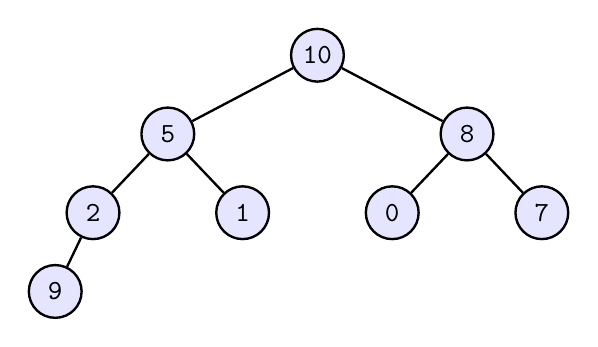
\begin{tikzpicture}

\fill[blue!10] (0.0, 0.0) circle (0.35);
\node [line width=0.03cm,black,minimum size=0.6699999999999999cm,draw,circle] at (0.0,0.0)(10){};\draw (0.0, 0.0) node[color=black] {\texttt{10}};
\fill[blue!10] (-1.9, -1.0) circle (0.35);
\node [line width=0.03cm,black,minimum size=0.6699999999999999cm,draw,circle] at (-1.9,-1.0)(5){};\draw (-1.9, -1.0) node[color=black] {\texttt{5}};
\fill[blue!10] (1.9, -1.0) circle (0.35);
\node [line width=0.03cm,black,minimum size=0.6699999999999999cm,draw,circle] at (1.9,-1.0)(8){};\draw (1.9, -1.0) node[color=black] {\texttt{8}};
\fill[blue!10] (-2.85, -2.0) circle (0.35);
\node [line width=0.03cm,black,minimum size=0.6699999999999999cm,draw,circle] at (-2.85,-2.0)(2){};\draw (-2.85, -2.0) node[color=black] {\texttt{2}};
\fill[blue!10] (-0.95, -2.0) circle (0.35);
\node [line width=0.03cm,black,minimum size=0.6699999999999999cm,draw,circle] at (-0.95,-2.0)(1){};\draw (-0.95, -2.0) node[color=black] {\texttt{1}};
\fill[blue!10] (0.95, -2.0) circle (0.35);
\node [line width=0.03cm,black,minimum size=0.6699999999999999cm,draw,circle] at (0.95,-2.0)(0){};\draw (0.95, -2.0) node[color=black] {\texttt{0}};
\fill[blue!10] (2.85, -2.0) circle (0.35);
\node [line width=0.03cm,black,minimum size=0.6699999999999999cm,draw,circle] at (2.85,-2.0)(7){};\draw (2.85, -2.0) node[color=black] {\texttt{7}};
\fill[blue!10] (-3.33, -3.0) circle (0.35);
\node [line width=0.03cm,black,minimum size=0.6699999999999999cm,draw,circle] at (-3.33,-3.0)(9){};\draw (-3.33, -3.0) node[color=black] {\texttt{9}};\draw[line width=0.03cm,black] (10) to  (5);
\draw[line width=0.03cm,black] (10) to  (8);
\draw[line width=0.03cm,black] (5) to  (2);
\draw[line width=0.03cm,black] (5) to  (1);
\draw[line width=0.03cm,black] (8) to  (0);
\draw[line width=0.03cm,black] (8) to  (7);
\draw[line width=0.03cm,black] (2) to  (9);
\end{tikzpicture}

\end{center}



It's easy to see that in the DFA, the $a$--
and $b$--transitions from the state $\{\}$ goes back to itself.
Therefore the completed DFA is this:


\begin{center}
\begin{tikzpicture}[>=triangle 60,shorten >=0.5pt,node distance=2cm,auto,initial text=, double distance=2pt]
\node[state,initial] (A) at (  0,  0) {$\{q_0\}$};
\node[state] (B) at (  3,  0) {$\{\}$};

\path[->]
(A) edge [bend left=0,pos=0.5,above] node {$a,b$} (B)
(B) edge [loop above] node {$a,b$} ()

;
\end{tikzpicture}
\end{center}
    



\newpage

Solution to Exercise \ref{ex:dfa-as-powerful-as-nfa1}\labeltext{}{sol:dfa-as-powerful-as-nfa1}.

\tinysidebar{\debug{exercises/{dfa-as-powerful-as-nfa1/answer.tex}}}

    Solution not provided.
    

\newpage

Solution to Exercise \ref{ex:dfa-as-powerful-as-nfa2}\labeltext{}{sol:dfa-as-powerful-as-nfa2}.

\tinysidebar{\debug{exercises/{dfa-as-powerful-as-nfa2/answer.tex}}}

    Solution not provided.
    

\newpage

Solution to Exercise \ref{ex:dfa-as-powerful-as-nfa3}\labeltext{}{sol:dfa-as-powerful-as-nfa3}.

\tinysidebar{\debug{exercises/{dfa-as-powerful-as-nfa3/answer.tex}}}

    Solution not provided.
    

\newpage

Solution to Exercise \ref{ex:dfa-as-powerful-as-nfa4}\labeltext{}{sol:dfa-as-powerful-as-nfa4}.

\tinysidebar{\debug{exercises/{dfa-as-powerful-as-nfa4/answer.tex}}}

    Solution not provided.
    

\newpage

Solution to Exercise \ref{ex:closure0}\labeltext{}{sol:closure0}.

\tinysidebar{\debug{exercises/{closure0/answer.tex}}}

    Solution not provided.
    

\newpage

Solution to Exercise \ref{ex:closure1}\labeltext{}{sol:closure1}.

\tinysidebar{\debug{exercises/{closure1/answer.tex}}}

    Solution not provided.
    

\newpage

Solution to Exercise \ref{ex:closure2}\labeltext{}{sol:closure2}.

\tinysidebar{\debug{exercises/{closure2/answer.tex}}}

    Solution not provided.
    

\newpage

Solution to Exercise \ref{ex:closure3}\labeltext{}{sol:closure3}.

\tinysidebar{\debug{exercises/{closure3/answer.tex}}}

    Solution not provided.
    

\newpage

Solution to Exercise \ref{ex:closure4}\labeltext{}{sol:closure4}.

\tinysidebar{\debug{exercises/{closure4/answer.tex}}}

    Solution not provided.
    

\newpage

Solution to Exercise \ref{ex:closure5}\labeltext{}{sol:closure5}.

\tinysidebar{\debug{exercises/{closure5/answer.tex}}}

    Solution not provided.
    

\newpage

Solution to Exercise \ref{ex:closure6}\labeltext{}{sol:closure6}.

\tinysidebar{\debug{exercises/{closure6/answer.tex}}}

    Solution not provided.
    

\newpage

Solution to Exercise \ref{ex:closure7}\labeltext{}{sol:closure7}.

\tinysidebar{\debug{exercises/{closure7/answer.tex}}}

    Solution not provided.
    

\newpage

Solution to Exercise \ref{ex:closure8}\labeltext{}{sol:closure8}.

\tinysidebar{\debug{exercises/{closure8/answer.tex}}}

    Solution not provided.
    

\newpage

Solution to Exercise \ref{ex:closure9}\labeltext{}{sol:closure9}.

\tinysidebar{\debug{exercises/{closure9/answer.tex}}}

    Solution not provided.
    

\newpage

Solution to Exercise \ref{ex:closure10}\labeltext{}{sol:closure10}.

\tinysidebar{\debug{exercises/{closure10/answer.tex}}}

    Solution not provided.
    

\newpage

Solution to Exercise \ref{ex:closure11}\labeltext{}{sol:closure11}.

\tinysidebar{\debug{exercises/{closure11/answer.tex}}}

    Solution not provided.
    

\newpage

Solution to Exercise \ref{ex:closure12}\labeltext{}{sol:closure12}.

\tinysidebar{\debug{exercises/{closure12/answer.tex}}}

    Solution not provided.
    

\begin{python0}
from solutions import *
clear()
\end{python0}
